% Figure 1 (overview), single column. Standalone TikZ, included at \columnwidth.
% Attention-edge matrix of one pooled prompt: rows are receiving tokens, columns are sending (earlier) tokens
% (Sam = source B, Alex = source A). Cells are coloured by the kind of attention edge that the paper's
% interventions remove; they are not attention weights.
% Accuracies: fig_overview_data.tex (scripts/fig_overview_data.py, E132).
\documentclass[11pt]{standalone}
\usepackage{times}
\usepackage[T1]{fontenc}
\usepackage{amssymb}
\usepackage{xcolor}
\usepackage{tikz}
\usetikzlibrary{arrows.meta,calc,patterns}
% Generated by scripts/fig_overview_data.py from numbers.json (E132); do not edit.
\def\accNative{72.1,85.9,72.5,71.3,58.8,71.1,72.7,79.3}
\def\meanNative{72.9}
\def\accIsolated{51.0,49.4,52.5,52.1,51.2,52.5,51.6,52.0}
\def\meanIsolated{51.5}
\def\accNames{73.2,78.1,80.3,70.9,69.5,87.9,67.2,84.8}
\def\meanNames{76.5}
\def\accSelective{87.5,96.1,93.8,85.2,80.1,98.0,80.7,93.9}
\def\meanSelective{89.4}


\definecolor{srcA}{HTML}{2F6DB3}
\definecolor{srcB}{HTML}{E08A2C}
\definecolor{nameC}{HTML}{3C9A64}
\definecolor{ink}{HTML}{262626}

% token i -> source (1 Sam, 2 Alex, 3 query) and field (1 comment, 2 name, 3 label)
\newcommand\tsec[1]{\ifcase#1\or1\or1\or1\or2\or2\or2\or3\or3\or3\fi}
\newcommand\tfld[1]{\ifcase#1\or1\or2\or3\or1\or2\or3\or1\or2\or3\fi}

% \drawmask{cell}{edges kept from Alex to Sam: 0 all, 1 none, 2 names only, 3 all but answer->label}
%          {1 if the query's edges to Sam are removed (A-only reading)}{gap}
\newcommand\drawmask[4]{%
  \foreach \i in {1,...,9} {
    \foreach \j in {1,...,\i} {
      \edef\sI{\tsec{\i}}\edef\sJ{\tsec{\j}}\edef\rJ{\tfld{\j}}\edef\rI{\tfld{\i}}
      \def\cc{white}\def\hatch{0}
      \ifnum\sI=\sJ
        \ifnum\sI=1 \def\cc{srcB!24}\fi
        \ifnum\sI=2 \def\cc{srcA!22}\fi
        \ifnum\sI=3 \def\cc{gray!22}\fi
      \else
        \ifnum\sI=2
          \def\cc{gray!32}
          \ifnum\rJ=2 \def\cc{nameC!65}\fi
          \ifnum\rJ=3 \ifnum\rI=3 \def\cc{srcB}\fi\fi
          \ifnum#2=1 \def\cc{white}\fi
          \ifnum#2=2 \ifnum\rJ=2 \else \def\cc{white}\fi\fi
          \ifnum#2=3 \ifnum\rJ=3 \ifnum\rI=3 \def\cc{white}\fi\fi\fi
        \fi
        \ifnum\sI=3
          \ifnum\sJ=1 \def\cc{gray!22}\ifnum#3=1 \def\cc{white}\def\hatch{1}\fi\fi
          \ifnum\sJ=2 \def\cc{srcA!35}\fi
        \fi
      \fi
      \fill[\cc] ({(\j-1)*#1+#4},{-(\i-1)*#1-#4}) rectangle ({\j*#1-#4},{-\i*#1+#4});
      \ifnum\hatch=1
        \fill[pattern=north east lines, pattern color=gray!50] ({(\j-1)*#1+#4},{-(\i-1)*#1-#4}) rectangle ({\j*#1-#4},{-\i*#1+#4});
      \fi
    }
  }
  \ifnum#2=1 \else
  % the query's final token reads Alex's label state, which carries Sam's rule
  \begin{scope}
    \clip ({5*#1+#4},{-8*#1-#4}) rectangle ({6*#1-#4},{-9*#1+#4});
    \fill[srcA] ({5*#1},{-8*#1}) rectangle ({6*#1},{-9*#1});
    \ifnum#2=3 \else
    \fill[srcB] ({6*#1},{-8*#1}) -- ({6*#1},{-9*#1}) -- ({5.3*#1},{-9*#1}) -- cycle;
    \fi
  \end{scope}
  \fi
}

\begin{document}
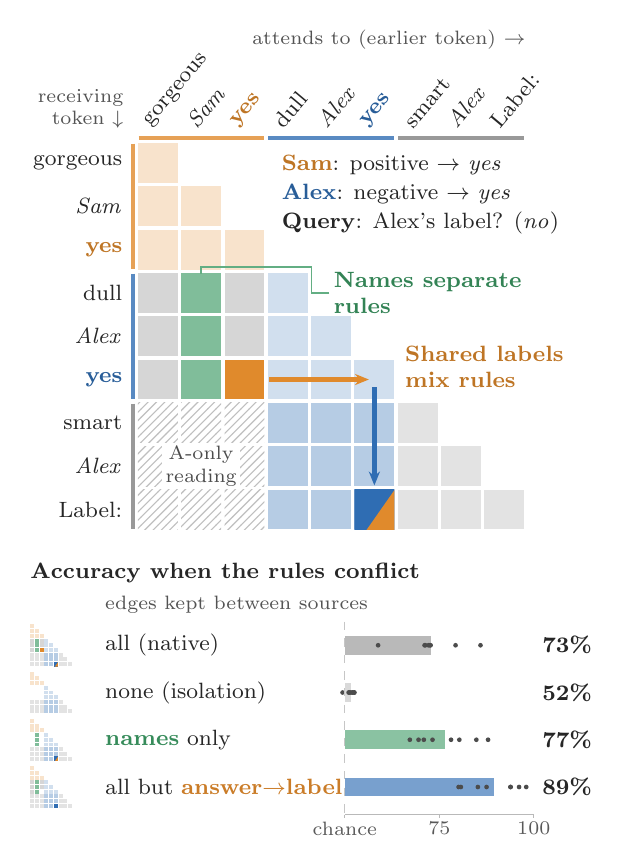
\begin{tikzpicture}[font=\footnotesize, text=ink,
  num/.style={circle, fill=white, draw=#1, text=#1, line width=.6pt, inner sep=0pt, minimum size=7.6pt,
              font=\fontsize{5.5}{6}\selectfont\bfseries},
  note/.style={anchor=north west, align=left, inner sep=0pt}]
\def\s{.55}
\drawmask{\s}{0}{1}{.022}

% ---------------- tokens ----------------
\foreach \j/\w/\c in {1/gorgeous/ink, 2/\textit{Sam}/ink, 3/\textbf{yes}/srcB!85!black,
                      4/dull/ink, 5/\textit{Alex}/ink, 6/\textbf{yes}/srcA!85!black,
                      7/smart/ink, 8/\textit{Alex}/ink, 9/Label:/ink} {
  \node[anchor=south west, rotate=50, inner sep=1pt, text=\c] at ({(\j-.5)*\s-.05},.09) {\w};
  \node[anchor=east, inner sep=2pt, text=\c] at (-.1,{-(\j-.5)*\s}) {\w};
}
\foreach \a/\b/\c in {1/3/srcB, 4/6/srcA, 7/9/gray} {
  \draw[\c!80, line width=1.6pt] ({(\a-1)*\s+.03},.04) -- ({\b*\s-.03},.04);
  \draw[\c!80, line width=1.6pt] (-.04,{-(\a-1)*\s-.03}) -- (-.04,{-\b*\s+.03});
}
% who follows which rule (key in the empty upper triangle)
\node[anchor=north west, align=left, inner sep=0pt] at ({3.35*\s},{-.3*\s}) {%
  \textcolor{srcB!85!black}{\textbf{Sam}}: positive $\to$ \textit{yes}\\[1pt]
  \textcolor{srcA!85!black}{\textbf{Alex}}: negative $\to$ \textit{yes}\\[1pt]
  \textbf{Query}: Alex's label? (\textit{no})};
\node[font=\scriptsize, text=gray!65!black, anchor=south east, align=right, inner sep=1pt] at (-.12,.12) {receiving\\token $\downarrow$};
\node[font=\scriptsize, text=gray!65!black, anchor=south west, inner sep=1pt] at ({2.6*\s},{1.12}) {attends to (earlier token) $\to$};

% ---------------- the path of Sam's rule ----------------
\draw[-{Stealth[length=5pt, width=4pt]}, line width=1.6pt, srcB] ({3*\s+.04},{-5.5*\s}) -- ({5.5*\s-.07},{-5.5*\s});
\draw[-{Stealth[length=5pt, width=4pt]}, line width=1.6pt, srcA] ({5.5*\s},{-5.5*\s-.1}) -- ({5.5*\s},{-8*\s+.03});

% ---------------- two labels, one tag ----------------
\node[anchor=west, align=left, inner sep=0pt, text=srcB!85!black, font=\footnotesize\bfseries] at ({6.2*\s},{-5.2*\s}) {Shared labels\\mix rules};
\node[anchor=west, align=left, inner sep=0pt, text=nameC!85!black, font=\footnotesize\bfseries] (nm) at ({4.55*\s},{-3.5*\s}) {Names separate\\rules};
\draw[nameC!80, line width=.6pt] ($(nm.west)+(-.05,0)$) -- ({4.05*\s},{-3.5*\s}) -- ({4.05*\s},{-2.9*\s}) -- ({1.5*\s},{-2.9*\s}) -- ({1.5*\s},{-3*\s-.04});
\node[fill=white, inner sep=1.2pt, font=\scriptsize, text=gray!60!black, align=center] at ({1.5*\s},{-7.5*\s}) {A-only\\reading};

% ---------------- interventions on formation: accuracy when the rules conflict ----------------
\begin{scope}[shift={(-1.35,-5.35)}]
  \def\L{2.4}
  \pgfmathsetmacro{\u}{\L/50}
  \def\bx{4.0}
  \node[anchor=north west, font=\footnotesize\bfseries, inner sep=0pt] at (0,0) {Accuracy when the rules conflict};
  \node[anchor=north west, font=\scriptsize, text=gray!65!black, inner sep=0pt] at (.95,-.42) {edges kept between sources};
  \foreach \row/\mode/\y/\lbl/\col in {
      Native/0/-1.05/{all (native)}/gray!55,
      Isolated/1/-1.65/{none (isolation)}/gray!30,
      Names/2/-2.25/{\textcolor{nameC!90!black}{\textbf{names}} only}/nameC!60,
      Selective/3/-2.85/{all but \textcolor{srcB!90!black}{\textbf{answer$\to$label}}}/srcA!65} {
    \begin{scope}[shift={(0,\y+.27)}] \drawmask{.06}{\mode}{0}{.005} \end{scope}
    \node[anchor=west, inner sep=0pt, font=\footnotesize] at (.95,\y) {\lbl};
    \pgfmathsetmacro{\m}{\csname mean\row\endcsname}
    \fill[\col] (\bx,\y-.12) rectangle ({\bx+(\m-50)*\u},\y+.12);
    \edef\lst{\csname acc\row\endcsname}
    \foreach \v in \lst \fill[black!70] ({\bx+(\v-50)*\u},\y) circle (.85pt);
    \pgfmathtruncatemacro{\mi}{round(\m)}
    \node[anchor=west, font=\footnotesize\bfseries, inner sep=0pt] at (\bx+\L+.1,\y) {\mi\%};
  }
  \draw[gray!55, line width=.4pt] (\bx,-3.2) -- (\bx+\L,-3.2);
  \foreach \t/\tl in {50/chance, 75/75, 100/100}
    \draw[gray!55, line width=.4pt] ({\bx+(\t-50)*\u},-3.2) -- ++(0,-.05) node[below, font=\scriptsize, text=gray!70!black, inner sep=1pt] {\tl};
  \draw[gray!45, dashed, line width=.4pt] (\bx,-.75) -- (\bx,-3.2);
\end{scope}

\end{tikzpicture}
\end{document}
